% Extended abstract for the IWH workshop (Halle). Every number in the text, table and captions comes from
% A_numeros_macros.tex, generated by R/A6_saidas.R from the CSV files in data/processed and results.
% Compile from results/: latexmk -pdf -auxdir=latex_aux -emulate-aux-dir A_extended_abstract.tex
\documentclass[11pt,a4paper]{article}
\usepackage[T1]{fontenc}
\usepackage[utf8]{inputenc}
\usepackage{lmodern}
\usepackage[margin=2.5cm]{geometry}
\usepackage{microtype}
\usepackage{amsmath}
\usepackage{booktabs}
\usepackage{graphicx}
\usepackage[round]{natbib}
\usepackage{url}
\usepackage{caption}
\usepackage{multicol}
\usepackage{titlesec}
\captionsetup{font=small,labelfont=sc,skip=3pt}
\titlespacing*{\section}{0pt}{1.4ex plus 0.4ex}{0.6ex}
\titleformat*{\section}{\large\bfseries}
\setlength{\bibsep}{0pt}
\setlength{\columnsep}{1.2em}
\setlength{\textfloatsep}{6pt plus 2pt}
\setlength{\floatsep}{6pt plus 2pt}

% Gerado por R/A6_saidas.R em 2026-09-29 00:30. Nao editar a mao. Formato ingles (ponto decimal).
% Cada macro traz, em comentario, o arquivo de origem.
\newcommand{\SampleStartYear}{2003} % data/processed/A3_invpub_trimestral.csv
\newcommand{\SampleEndYear}{2025} % data/processed/A3_invpub_trimestral.csv
\newcommand{\SampleFull}{2003Q1--2025Q4} % data/processed/A5_lp_cumulativo.csv
\newcommand{\NQuarters}{92} % data/processed/A2_series_trimestrais.csv
\newcommand{\SampleOrig}{2002--2019} % data/processed/A5_var_resultados.csv
\newcommand{\SampleCorr}{2003--2019} % data/processed/A5_var_resultados.csv
\newcommand{\SampleExt}{2003--2025} % data/processed/A5_var_resultados.csv
\newcommand{\CILevel}{90} % data/processed/A5_lp_cumulativo.csv
\newcommand{\SigLevel}{5} % data/processed/A5_johansen.csv
\newcommand{\SigLevelTen}{10} % data/processed/A5_lp_comparacoes.csv
\newcommand{\VARp}{3} % data/processed/A5_var_resultados.csv
\newcommand{\VARh}{40} % data/processed/A5_var_resultados.csv
\newcommand{\VARruns}{2000} % data/processed/A5_var_resultados.csv
\newcommand{\JohK}{3} % data/processed/A5_johansen.csv
\newcommand{\JohB}{999} % data/processed/A5_johansen.csv
\newcommand{\LPp}{3} % data/processed/A5_lp_cumulativo.csv
\newcommand{\LPpShort}{2} % data/processed/A5_lp_cumulativo.csv
\newcommand{\LPhmax}{12} % data/processed/A5_lp_irf.csv
\newcommand{\LPhmaxShort}{8} % data/processed/A5_lp_irf.csv
\newcommand{\hA}{4} % data/processed/A5_lp_cumulativo.csv
\newcommand{\hB}{8} % data/processed/A5_lp_cumulativo.csv
\newcommand{\hC}{12} % data/processed/A5_lp_cumulativo.csv
\newcommand{\nLPA}{84} % data/processed/A5_lp_cumulativo.csv
\newcommand{\nLPC}{76} % data/processed/A5_lp_cumulativo.csv
\newcommand{\nLPzero}{88} % data/processed/A5_lp_irf.csv
\newcommand{\PulseDates}{2020Q2 and 2020Q3} % data/processed/A4_dummies_quebra.csv
\newcommand{\PerShares}{2003--2025} % data/processed/A3_invpub_trimestral.csv
\newcommand{\ShareSocTransf}{70} % data/processed/A3_invpub_trimestral.csv
\newcommand{\ShareEconDir}{92} % data/processed/A3_invpub_trimestral.csv
\newcommand{\SestBoletimEnd}{2019} % data/processed/A3_invpub_trimestral.csv
\newcommand{\SestOIStart}{2016} % data/processed/A3_invpub_trimestral.csv
\newcommand{\PetroShareMin}{82} % data/processed/A3_invpub_trimestral.csv
\newcommand{\PetroShareMax}{91} % data/processed/A3_invpub_trimestral.csv
\newcommand{\PerOI}{2016--2025} % data/processed/A3_invpub_trimestral.csv
\newcommand{\BaseYear}{2025} % data/processed/A3_invpub_trimestral.csv
\newcommand{\nRep}{68} % data/processed/A5_var_resultados.csv
\newcommand{\nCorr}{64} % data/processed/A5_var_resultados.csv
\newcommand{\nExt}{88} % data/processed/A5_var_resultados.csv
\newcommand{\ImpRep}{0.0118} % data/processed/A5_var_resultados.csv
\newcommand{\AcumRep}{0.0194} % data/processed/A5_var_resultados.csv
\newcommand{\AcumInfRep}{0.0465} % data/processed/A5_var_resultados.csv
\newcommand{\ElastRep}{0.42} % data/processed/A5_var_resultados.csv
\newcommand{\ElastRepLo}{0.05} % data/processed/A5_var_resultados.csv
\newcommand{\ElastRepHi}{0.66} % data/processed/A5_var_resultados.csv
\newcommand{\ElastCorr}{0.45} % data/processed/A5_var_resultados.csv
\newcommand{\ElastCorrLo}{0.10} % data/processed/A5_var_resultados.csv
\newcommand{\ElastCorrHi}{0.69} % data/processed/A5_var_resultados.csv
\newcommand{\ElastExt}{0.17} % data/processed/A5_var_resultados.csv
\newcommand{\ElastExtLo}{\ensuremath{-}0.03} % data/processed/A5_var_resultados.csv
\newcommand{\ElastExtHi}{0.36} % data/processed/A5_var_resultados.csv
\newcommand{\pGrangerRep}{0.024} % data/processed/A5_var_resultados.csv
\newcommand{\pGrangerRevRep}{0.29} % data/processed/A5_var_resultados.csv
\newcommand{\pGrangerTextRev}{0.56} % data/processed/A1_alvos_dissertacao.csv
\newcommand{\FGrangerTextRev}{1.90} % data/processed/A1_alvos_dissertacao.csv
\newcommand{\pGrangerImplied}{0.13} % data/processed/A1_alvos_dissertacao.csv
\newcommand{\JohTextTrace}{25.01} % data/processed/A1_alvos_dissertacao.csv
\newcommand{\JohTextCV}{25.32} % data/processed/A1_alvos_dissertacao.csv
\newcommand{\DumDates}{2018Q2--2019Q1 and 2019Q3--2019Q4} % data/original/0124_inexo.txt
\newcommand{\CorrNominal}{0.997} % results/A3_reconstrucao_INF_variantes.csv
\newcommand{\DevNominal}{0.005} % results/A3_reconstrucao_INF_variantes.csv
\newcommand{\CorrReal}{0.995} % results/A3_reconstrucao_INF_variantes.csv
\newcommand{\DevReal}{0.19} % results/A3_reconstrucao_INF_variantes.csv
\newcommand{\JohTrOrig}{24.19} % data/processed/A5_johansen.csv
\newcommand{\JohRaOrig}{22.09} % data/processed/A5_johansen.csv
\newcommand{\JohBootOrig}{0.170} % data/processed/A5_johansen.csv
\newcommand{\VecOrig}{0.58} % data/processed/A5_var_resultados.csv
\newcommand{\VecOrigLo}{0.42} % data/processed/A5_var_resultados.csv
\newcommand{\VecOrigHi}{0.82} % data/processed/A5_var_resultados.csv
\newcommand{\JohTrCorr}{28.79} % data/processed/A5_johansen.csv
\newcommand{\JohRaCorr}{26.13} % data/processed/A5_johansen.csv
\newcommand{\JohBootCorr}{0.086} % data/processed/A5_johansen.csv
\newcommand{\VecCorr}{0.55} % data/processed/A5_var_resultados.csv
\newcommand{\VecCorrLo}{0.40} % data/processed/A5_var_resultados.csv
\newcommand{\VecCorrHi}{0.76} % data/processed/A5_var_resultados.csv
\newcommand{\JohTrExt}{26.29} % data/processed/A5_johansen.csv
\newcommand{\JohRaExt}{24.52} % data/processed/A5_johansen.csv
\newcommand{\JohBootExt}{0.124} % data/processed/A5_johansen.csv
\newcommand{\VecExt}{0.51} % data/processed/A5_var_resultados.csv
\newcommand{\VecExtLo}{0.36} % data/processed/A5_var_resultados.csv
\newcommand{\VecExtHi}{0.66} % data/processed/A5_var_resultados.csv
\newcommand{\JohCV}{25.32} % data/processed/A5_johansen.csv
\newcommand{\ElastCholCorr}{0.07} % data/processed/A5_var_resultados.csv
\newcommand{\ElastCholCorrLo}{\ensuremath{-}0.25} % data/processed/A5_var_resultados.csv
\newcommand{\ElastCholCorrHi}{0.30} % data/processed/A5_var_resultados.csv
\newcommand{\ElastCholExt}{0.14} % data/processed/A5_var_resultados.csv
\newcommand{\ElastCholExtLo}{\ensuremath{-}0.00} % data/processed/A5_var_resultados.csv
\newcommand{\ElastCholExtHi}{0.27} % data/processed/A5_var_resultados.csv
\newcommand{\ElastPtwoCorr}{0.06} % data/processed/A5_var_resultados.csv
\newcommand{\ElastPtwoCorrLo}{\ensuremath{-}0.25} % data/processed/A5_var_resultados.csv
\newcommand{\ElastPtwoCorrHi}{0.31} % data/processed/A5_var_resultados.csv
\newcommand{\ElastPtwoExt}{0.11} % data/processed/A5_var_resultados.csv
\newcommand{\ElastPtwoExtLo}{\ensuremath{-}0.08} % data/processed/A5_var_resultados.csv
\newcommand{\ElastPtwoExtHi}{0.28} % data/processed/A5_var_resultados.csv
\newcommand{\ElastGdpCorr}{0.23} % data/processed/A5_var_resultados.csv
\newcommand{\ElastGdpCorrLo}{0.02} % data/processed/A5_var_resultados.csv
\newcommand{\ElastGdpCorrHi}{0.39} % data/processed/A5_var_resultados.csv
\newcommand{\ElastGdpExt}{0.10} % data/processed/A5_var_resultados.csv
\newcommand{\ElastGdpExtLo}{\ensuremath{-}0.06} % data/processed/A5_var_resultados.csv
\newcommand{\ElastGdpExtHi}{0.24} % data/processed/A5_var_resultados.csv
\newcommand{\ElastSubA}{0.23} % data/processed/A5_var_resultados.csv
\newcommand{\ElastSubALo}{\ensuremath{-}0.37} % data/processed/A5_var_resultados.csv
\newcommand{\ElastSubAHi}{0.53} % data/processed/A5_var_resultados.csv
\newcommand{\ElastSubB}{0.06} % data/processed/A5_var_resultados.csv
\newcommand{\ElastSubBLo}{\ensuremath{-}0.17} % data/processed/A5_var_resultados.csv
\newcommand{\ElastSubBHi}{0.26} % data/processed/A5_var_resultados.csv
\newcommand{\SubAEnd}{2014Q4} % data/processed/A5_var_resultados.csv
\newcommand{\SubBStart}{2015Q1} % data/processed/A5_var_resultados.csv
\newcommand{\ElastDumA}{0.34} % data/processed/A5_var_resultados.csv
\newcommand{\ElastDumALo}{0.12} % data/processed/A5_var_resultados.csv
\newcommand{\ElastDumAHi}{0.55} % data/processed/A5_var_resultados.csv
\newcommand{\SupFDate}{2020Q2} % results/A4_quebras_resumo.csv
\newcommand{\SupFpInf}{0.013} % results/A4_quebras_resumo.csv
\newcommand{\SupFpFbcf}{\ensuremath{<}0.001} % results/A4_quebras_resumo.csv
\newcommand{\LpInfElast}{0.10} % data/processed/A5_lp_cumulativo.csv
\newcommand{\LpInfElastLo}{\ensuremath{-}0.05} % data/processed/A5_lp_cumulativo.csv
\newcommand{\LpInfElastHi}{0.25} % data/processed/A5_lp_cumulativo.csv
\newcommand{\LpInfMult}{1.83} % data/processed/A5_lp_cumulativo.csv
\newcommand{\LpInfMultLo}{0.19} % data/processed/A5_lp_cumulativo.csv
\newcommand{\LpInfMultHi}{3.47} % data/processed/A5_lp_cumulativo.csv
\newcommand{\LpSoeMult}{1.83} % data/processed/A5_lp_cumulativo.csv
\newcommand{\LpSoeMultLo}{\ensuremath{-}0.12} % data/processed/A5_lp_cumulativo.csv
\newcommand{\LpSoeMultHi}{3.79} % data/processed/A5_lp_cumulativo.csv
\newcommand{\LpGndElast}{0.28} % data/processed/A5_lp_cumulativo.csv
\newcommand{\LpGndElastLo}{0.08} % data/processed/A5_lp_cumulativo.csv
\newcommand{\LpGndElastHi}{0.47} % data/processed/A5_lp_cumulativo.csv
\newcommand{\LpGndMultB}{5.96} % data/processed/A5_lp_cumulativo.csv
\newcommand{\LpGndMultBLo}{1.04} % data/processed/A5_lp_cumulativo.csv
\newcommand{\LpGndMultBHi}{10.88} % data/processed/A5_lp_cumulativo.csv
\newcommand{\LpGndMult}{6.64} % data/processed/A5_lp_cumulativo.csv
\newcommand{\LpGndMultLo}{\ensuremath{-}0.60} % data/processed/A5_lp_cumulativo.csv
\newcommand{\LpGndMultHi}{13.87} % data/processed/A5_lp_cumulativo.csv
\newcommand{\LpSocDirMultSep}{49.5} % data/processed/A5_lp_cumulativo.csv
\newcommand{\LpSocDirMultJoint}{13.6} % data/processed/A5_lp_comparacoes.csv
\newcommand{\LpSocDirMultJointLo}{\ensuremath{-}30.4} % data/processed/A5_lp_comparacoes.csv
\newcommand{\LpSocDirMultJointHi}{57.7} % data/processed/A5_lp_comparacoes.csv
\newcommand{\GshareInf}{7.4} % data/processed/A3_niveis_wide.csv
\newcommand{\GshareSoe}{5.8} % data/processed/A3_niveis_wide.csv
\newcommand{\GshareSocDir}{0.3} % data/processed/A3_niveis_wide.csv
\newcommand{\GshareEconDir}{0.8} % data/processed/A3_niveis_wide.csv
\newcommand{\GshareTransfSoc}{0.8} % data/processed/A3_niveis_wide.csv
\newcommand{\NexclZero}{84} % data/processed/A5_lp_cumulativo.csv
\newcommand{\NcumTotal}{264} % data/processed/A5_lp_cumulativo.csv
\newcommand{\EcoSocDirHAA}{0.02} % data/processed/A5_lp_comparacoes.csv
\newcommand{\EcoSocDirHAB}{0.09} % data/processed/A5_lp_comparacoes.csv
\newcommand{\EcoSocDirHAp}{0.396} % data/processed/A5_lp_comparacoes.csv
\newcommand{\EcoSocDirHApUnadj}{0.338} % data/processed/A5_lp_comparacoes.csv
\newcommand{\EcoSocDirHAn}{84} % data/processed/A5_lp_comparacoes.csv
\newcommand{\EcoSocDirHAdf}{67} % data/processed/A5_lp_comparacoes.csv
\newcommand{\EcoSocDirHAMEp}{0.893} % data/processed/A5_lp_comparacoes.csv
\newcommand{\EcoSocDirHAAe}{0.02} % data/processed/A5_lp_comparacoes.csv
\newcommand{\EcoSocDirHAAeLo}{\ensuremath{-}0.04} % data/processed/A5_lp_comparacoes.csv
\newcommand{\EcoSocDirHAAeHi}{0.07} % data/processed/A5_lp_comparacoes.csv
\newcommand{\EcoSocDirHABe}{0.09} % data/processed/A5_lp_comparacoes.csv
\newcommand{\EcoSocDirHABeLo}{\ensuremath{-}0.02} % data/processed/A5_lp_comparacoes.csv
\newcommand{\EcoSocDirHABeHi}{0.20} % data/processed/A5_lp_comparacoes.csv
\newcommand{\EcoSocDirHCA}{0.08} % data/processed/A5_lp_comparacoes.csv
\newcommand{\EcoSocDirHCB}{0.04} % data/processed/A5_lp_comparacoes.csv
\newcommand{\EcoSocDirHCp}{0.817} % data/processed/A5_lp_comparacoes.csv
\newcommand{\EcoSocDirHCpUnadj}{0.792} % data/processed/A5_lp_comparacoes.csv
\newcommand{\EcoSocDirHCn}{76} % data/processed/A5_lp_comparacoes.csv
\newcommand{\EcoSocDirHCdf}{59} % data/processed/A5_lp_comparacoes.csv
\newcommand{\EcoSocDirHCMEp}{0.439} % data/processed/A5_lp_comparacoes.csv
\newcommand{\EcoSocDirHCAe}{0.08} % data/processed/A5_lp_comparacoes.csv
\newcommand{\EcoSocDirHCAeLo}{\ensuremath{-}0.07} % data/processed/A5_lp_comparacoes.csv
\newcommand{\EcoSocDirHCAeHi}{0.22} % data/processed/A5_lp_comparacoes.csv
\newcommand{\EcoSocDirHCBe}{0.04} % data/processed/A5_lp_comparacoes.csv
\newcommand{\EcoSocDirHCBeLo}{\ensuremath{-}0.13} % data/processed/A5_lp_comparacoes.csv
\newcommand{\EcoSocDirHCBeHi}{0.20} % data/processed/A5_lp_comparacoes.csv
\newcommand{\EcoSocDtHAA}{0.05} % data/processed/A5_lp_comparacoes.csv
\newcommand{\EcoSocDtHAB}{\ensuremath{-}0.00} % data/processed/A5_lp_comparacoes.csv
\newcommand{\EcoSocDtHAp}{0.508} % data/processed/A5_lp_comparacoes.csv
\newcommand{\EcoSocDtHApUnadj}{0.456} % data/processed/A5_lp_comparacoes.csv
\newcommand{\EcoSocDtHAn}{84} % data/processed/A5_lp_comparacoes.csv
\newcommand{\EcoSocDtHAdf}{67} % data/processed/A5_lp_comparacoes.csv
\newcommand{\EcoSocDtHAMEp}{0.768} % data/processed/A5_lp_comparacoes.csv
\newcommand{\EcoSocDtHAAe}{0.05} % data/processed/A5_lp_comparacoes.csv
\newcommand{\EcoSocDtHAAeLo}{\ensuremath{-}0.02} % data/processed/A5_lp_comparacoes.csv
\newcommand{\EcoSocDtHAAeHi}{0.12} % data/processed/A5_lp_comparacoes.csv
\newcommand{\EcoSocDtHABe}{\ensuremath{-}0.00} % data/processed/A5_lp_comparacoes.csv
\newcommand{\EcoSocDtHABeLo}{\ensuremath{-}0.09} % data/processed/A5_lp_comparacoes.csv
\newcommand{\EcoSocDtHABeHi}{0.09} % data/processed/A5_lp_comparacoes.csv
\newcommand{\EcoSocDtHCA}{0.08} % data/processed/A5_lp_comparacoes.csv
\newcommand{\EcoSocDtHCB}{0.01} % data/processed/A5_lp_comparacoes.csv
\newcommand{\EcoSocDtHCp}{0.511} % data/processed/A5_lp_comparacoes.csv
\newcommand{\EcoSocDtHCpUnadj}{0.452} % data/processed/A5_lp_comparacoes.csv
\newcommand{\EcoSocDtHCn}{76} % data/processed/A5_lp_comparacoes.csv
\newcommand{\EcoSocDtHCdf}{59} % data/processed/A5_lp_comparacoes.csv
\newcommand{\EcoSocDtHCMEp}{0.609} % data/processed/A5_lp_comparacoes.csv
\newcommand{\EcoSocDtHCAe}{0.08} % data/processed/A5_lp_comparacoes.csv
\newcommand{\EcoSocDtHCAeLo}{\ensuremath{-}0.02} % data/processed/A5_lp_comparacoes.csv
\newcommand{\EcoSocDtHCAeHi}{0.19} % data/processed/A5_lp_comparacoes.csv
\newcommand{\EcoSocDtHCBe}{0.01} % data/processed/A5_lp_comparacoes.csv
\newcommand{\EcoSocDtHCBeLo}{\ensuremath{-}0.13} % data/processed/A5_lp_comparacoes.csv
\newcommand{\EcoSocDtHCBeHi}{0.15} % data/processed/A5_lp_comparacoes.csv
\newcommand{\SocTrHAA}{0.13} % data/processed/A5_lp_comparacoes.csv
\newcommand{\SocTrHAB}{0.00} % data/processed/A5_lp_comparacoes.csv
\newcommand{\SocTrHAp}{0.014} % data/processed/A5_lp_comparacoes.csv
\newcommand{\SocTrHApUnadj}{0.005} % data/processed/A5_lp_comparacoes.csv
\newcommand{\SocTrHAn}{84} % data/processed/A5_lp_comparacoes.csv
\newcommand{\SocTrHAdf}{67} % data/processed/A5_lp_comparacoes.csv
\newcommand{\SocTrHAMEp}{0.390} % data/processed/A5_lp_comparacoes.csv
\newcommand{\SocTrHAAe}{0.13} % data/processed/A5_lp_comparacoes.csv
\newcommand{\SocTrHAAeLo}{0.05} % data/processed/A5_lp_comparacoes.csv
\newcommand{\SocTrHAAeHi}{0.21} % data/processed/A5_lp_comparacoes.csv
\newcommand{\SocTrHABe}{0.00} % data/processed/A5_lp_comparacoes.csv
\newcommand{\SocTrHABeLo}{\ensuremath{-}0.05} % data/processed/A5_lp_comparacoes.csv
\newcommand{\SocTrHABeHi}{0.05} % data/processed/A5_lp_comparacoes.csv
\newcommand{\SocTrHBA}{0.14} % data/processed/A5_lp_comparacoes.csv
\newcommand{\SocTrHBB}{0.02} % data/processed/A5_lp_comparacoes.csv
\newcommand{\SocTrHBp}{0.061} % data/processed/A5_lp_comparacoes.csv
\newcommand{\SocTrHBpUnadj}{0.032} % data/processed/A5_lp_comparacoes.csv
\newcommand{\SocTrHBn}{80} % data/processed/A5_lp_comparacoes.csv
\newcommand{\SocTrHBdf}{63} % data/processed/A5_lp_comparacoes.csv
\newcommand{\SocTrHBMEp}{0.315} % data/processed/A5_lp_comparacoes.csv
\newcommand{\SocTrHBAe}{0.14} % data/processed/A5_lp_comparacoes.csv
\newcommand{\SocTrHBAeLo}{0.03} % data/processed/A5_lp_comparacoes.csv
\newcommand{\SocTrHBAeHi}{0.26} % data/processed/A5_lp_comparacoes.csv
\newcommand{\SocTrHBBe}{0.02} % data/processed/A5_lp_comparacoes.csv
\newcommand{\SocTrHBBeLo}{\ensuremath{-}0.02} % data/processed/A5_lp_comparacoes.csv
\newcommand{\SocTrHBBeHi}{0.07} % data/processed/A5_lp_comparacoes.csv
\newcommand{\SocTrHCA}{0.15} % data/processed/A5_lp_comparacoes.csv
\newcommand{\SocTrHCB}{0.02} % data/processed/A5_lp_comparacoes.csv
\newcommand{\SocTrHCp}{0.082} % data/processed/A5_lp_comparacoes.csv
\newcommand{\SocTrHCpUnadj}{0.044} % data/processed/A5_lp_comparacoes.csv
\newcommand{\SocTrHCn}{76} % data/processed/A5_lp_comparacoes.csv
\newcommand{\SocTrHCdf}{59} % data/processed/A5_lp_comparacoes.csv
\newcommand{\SocTrHCMEp}{0.454} % data/processed/A5_lp_comparacoes.csv
\newcommand{\SocTrHCAe}{0.15} % data/processed/A5_lp_comparacoes.csv
\newcommand{\SocTrHCAeLo}{0.03} % data/processed/A5_lp_comparacoes.csv
\newcommand{\SocTrHCAeHi}{0.26} % data/processed/A5_lp_comparacoes.csv
\newcommand{\SocTrHCBe}{0.02} % data/processed/A5_lp_comparacoes.csv
\newcommand{\SocTrHCBeLo}{\ensuremath{-}0.05} % data/processed/A5_lp_comparacoes.csv
\newcommand{\SocTrHCBeHi}{0.09} % data/processed/A5_lp_comparacoes.csv
\newcommand{\SoeHAA}{0.19} % data/processed/A5_lp_comparacoes.csv
\newcommand{\SoeHAB}{\ensuremath{-}0.04} % data/processed/A5_lp_comparacoes.csv
\newcommand{\SoeHAp}{0.017} % data/processed/A5_lp_comparacoes.csv
\newcommand{\SoeHApUnadj}{\ensuremath{<}0.001} % data/processed/A5_lp_comparacoes.csv
\newcommand{\SoeHAn}{33} % data/processed/A5_lp_comparacoes.csv
\newcommand{\SoeHAdf}{19} % data/processed/A5_lp_comparacoes.csv
\newcommand{\SoeHAMEp}{0.514} % data/processed/A5_lp_comparacoes.csv
\newcommand{\SoeHAAe}{0.19} % data/processed/A5_lp_comparacoes.csv
\newcommand{\SoeHAAeLo}{0.05} % data/processed/A5_lp_comparacoes.csv
\newcommand{\SoeHAAeHi}{0.33} % data/processed/A5_lp_comparacoes.csv
\newcommand{\SoeHABe}{\ensuremath{-}0.04} % data/processed/A5_lp_comparacoes.csv
\newcommand{\SoeHABeLo}{\ensuremath{-}0.08} % data/processed/A5_lp_comparacoes.csv
\newcommand{\SoeHABeHi}{\ensuremath{-}0.01} % data/processed/A5_lp_comparacoes.csv
\newcommand{\SoeHBA}{0.20} % data/processed/A5_lp_comparacoes.csv
\newcommand{\SoeHBB}{\ensuremath{-}0.07} % data/processed/A5_lp_comparacoes.csv
\newcommand{\SoeHBp}{0.016} % data/processed/A5_lp_comparacoes.csv
\newcommand{\SoeHBpUnadj}{\ensuremath{<}0.001} % data/processed/A5_lp_comparacoes.csv
\newcommand{\SoeHBn}{29} % data/processed/A5_lp_comparacoes.csv
\newcommand{\SoeHBdf}{15} % data/processed/A5_lp_comparacoes.csv
\newcommand{\SoeHBMEp}{0.176} % data/processed/A5_lp_comparacoes.csv
\newcommand{\SoeHBAe}{0.20} % data/processed/A5_lp_comparacoes.csv
\newcommand{\SoeHBAeLo}{0.02} % data/processed/A5_lp_comparacoes.csv
\newcommand{\SoeHBAeHi}{0.38} % data/processed/A5_lp_comparacoes.csv
\newcommand{\SoeHBBe}{\ensuremath{-}0.07} % data/processed/A5_lp_comparacoes.csv
\newcommand{\SoeHBBeLo}{\ensuremath{-}0.09} % data/processed/A5_lp_comparacoes.csv
\newcommand{\SoeHBBeHi}{\ensuremath{-}0.04} % data/processed/A5_lp_comparacoes.csv
\newcommand{\SoeUniHAA}{\ensuremath{-}0.02} % data/processed/A5_lp_comparacoes.csv
\newcommand{\SoeUniHAB}{0.12} % data/processed/A5_lp_comparacoes.csv
\newcommand{\SoeUniHAp}{0.141} % data/processed/A5_lp_comparacoes.csv
\newcommand{\SoeUniHApUnadj}{0.096} % data/processed/A5_lp_comparacoes.csv
\newcommand{\SoeUniHAn}{84} % data/processed/A5_lp_comparacoes.csv
\newcommand{\SoeUniHAdf}{67} % data/processed/A5_lp_comparacoes.csv
\newcommand{\SoeUniHAMEp}{0.248} % data/processed/A5_lp_comparacoes.csv
\newcommand{\SoeUniHAAe}{\ensuremath{-}0.02} % data/processed/A5_lp_comparacoes.csv
\newcommand{\SoeUniHAAeLo}{\ensuremath{-}0.11} % data/processed/A5_lp_comparacoes.csv
\newcommand{\SoeUniHAAeHi}{0.07} % data/processed/A5_lp_comparacoes.csv
\newcommand{\SoeUniHABe}{0.12} % data/processed/A5_lp_comparacoes.csv
\newcommand{\SoeUniHABeLo}{0.02} % data/processed/A5_lp_comparacoes.csv
\newcommand{\SoeUniHABeHi}{0.22} % data/processed/A5_lp_comparacoes.csv
\newcommand{\SoeUniHCA}{0.00} % data/processed/A5_lp_comparacoes.csv
\newcommand{\SoeUniHCB}{0.18} % data/processed/A5_lp_comparacoes.csv
\newcommand{\SoeUniHCp}{0.127} % data/processed/A5_lp_comparacoes.csv
\newcommand{\SoeUniHCpUnadj}{0.079} % data/processed/A5_lp_comparacoes.csv
\newcommand{\SoeUniHCn}{76} % data/processed/A5_lp_comparacoes.csv
\newcommand{\SoeUniHCdf}{59} % data/processed/A5_lp_comparacoes.csv
\newcommand{\SoeUniHCMEp}{0.139} % data/processed/A5_lp_comparacoes.csv
\newcommand{\SoeUniHCAe}{0.00} % data/processed/A5_lp_comparacoes.csv
\newcommand{\SoeUniHCAeLo}{\ensuremath{-}0.10} % data/processed/A5_lp_comparacoes.csv
\newcommand{\SoeUniHCAeHi}{0.11} % data/processed/A5_lp_comparacoes.csv
\newcommand{\SoeUniHCBe}{0.18} % data/processed/A5_lp_comparacoes.csv
\newcommand{\SoeUniHCBeLo}{0.04} % data/processed/A5_lp_comparacoes.csv
\newcommand{\SoeUniHCBeHi}{0.32} % data/processed/A5_lp_comparacoes.csv
\newcommand{\SocTrMEpMin}{0.315} % data/processed/A5_lp_comparacoes.csv
\newcommand{\SocTrMEpMax}{0.454} % data/processed/A5_lp_comparacoes.csv
\newcommand{\SoeUnipMin}{0.105} % data/processed/A5_lp_comparacoes.csv
\newcommand{\SoeUnipMax}{0.141} % data/processed/A5_lp_comparacoes.csv
\newcommand{\EcoSocpMin}{0.395} % data/processed/A5_lp_comparacoes.csv


\title{\vspace{-8ex}Which public investment crowds in private investment?\\ Evidence for Brazil by investor and type of infrastructure}
\author{Arthur Cassemiro Bispo\\[0.2ex]
  \small Institute of Economics, University of Campinas (Unicamp), Brazil\\
  \small Extended abstract, IWH workshop, Halle}
\date{\vspace{-5ex}}

\begin{document}
\maketitle
\vspace{-4ex}

\begin{abstract}
\noindent We revisit a quarterly VAR estimate for Brazil in which federal public investment raises private investment in machinery and equipment, and ask whether the effect depends on who invests and on what is built. The replication reproduces a long-run elasticity of \ElastRep{} (\CILevel\% CI \ElastRepLo{} to \ElastRepHi{}). After deflating public investment (the original series was nominal) and updating the data, the elasticity for \SampleCorr{} is \ElastCorr{} (\ElastCorrLo{} to \ElastCorrHi{}); it loses significance when the Cholesky order is reversed or two lags are used, and it falls to \ElastExt{} (\ElastExtLo{} to \ElastExtHi{}) in the sample extended to \SampleEndYear{}. Local projections on new series by investor and type of infrastructure find no difference between economic and social federal investment (all $p \geq \EcoSocpMin$). Direct federal social investment raises gross fixed capital formation more than capital transfers to states and municipalities ($p = \SocTrHAp$ after \hA{} quarters; \SocTrHBp{} and \SocTrHCp{} after \hB{} and \hC{}), and non-oil state-owned enterprises more than oil ($p = \SoeHAp$, $n = \SoeHAn$). Neither gap appears in machinery and equipment.
\end{abstract}
\vspace{-1.5ex}

\section{Motivation and question}

Brazilian estimates of the effect of public on private investment disagree: some studies find crowding-in \citep{reis2019, iasco2023} and others crowding-out \citep{jacinto1998, oliveira2020}. In a master's dissertation we estimated a quarterly VAR for \SampleOrig{} in which federal public investment (direct federal investment plus federal state-owned enterprises, SOEs) Granger-causes private investment in machinery and equipment and raises it in the long run, and we closed by proposing a more sectoral treatment of public investment. We now ask whether the effect depends on who invests (the federal government directly, the federal government through capital transfers to states and municipalities, or an SOE) and on what is built: economic infrastructure (transport, energy, communications) or social infrastructure (education, health, sanitation, housing and other social functions). We first replicate and correct the original estimate.


\section{Data}

All series are quarterly and cover \SampleFull{} (\NQuarters{} quarters). Federal investment is paid investment spending, including paid carry-overs, from SIAFI. We classify it by budget function into economic and social infrastructure and by modality into direct application and transfers to states and municipalities. The modality matters: over \PerShares{}, transfers carried \ShareSocTransf\% of federal investment in social infrastructure, while \ShareEconDir\% of economic infrastructure was direct application (nominal sums). SOE investment comes from the SOE investment bulletin up to \SestBoletimEnd{}, chained to the SOE investment budget, which from \SestOIStart{} separates oil and gas (\PetroShareMin\% to \PetroShareMax\% of SOE investment per year). Public series are in reais of \BaseYear{} (IPCA), adjusted with X-11 and entered as log indices. Private investment is the Ipea indicator of machinery and equipment (as in the dissertation) and gross fixed capital formation (GFCF) in volume from the quarterly national accounts.

\section{Empirical strategy}

\textit{VAR and VEC.} The original model is a VAR(\VARp) in first differences of log public investment and log machinery and equipment, with constant, trend and exogenous GDP, Selic and a dummy, and public investment first in a Cholesky ordering. The long-run elasticity is the ratio of the cumulative responses of private and public investment after \VARh{} quarters, with bootstrap intervals (\VARruns{} replications). To choose between the VAR in differences and a vector error correction (VEC) model we use Johansen's trace test with $K = \JohK$ \citep{johansen1991}, its small-sample version \citep{reinsel1992} and a wild bootstrap with \JohB{} replications \citep{cavaliere2012}; a rule set before estimation follows the bootstrap at the \SigLevel\% level and reports the VEC next to the VAR when the readings disagree.

\textit{Local projections.} For each public series $x$ and private series $y$ we project $y_{t+h}-y_{t-1}$ on $\Delta x_t$ \citep{jorda2005} for horizons up to \LPhmax{} quarters, with \LPp{} lags of both differences, constant, trend, GDP acceleration, the Selic and dummies for \PulseDates{}. The cumulative elasticity is the two-stage least squares coefficient of the summed response on the summed shock, instrumented by $\Delta x_t$; the multiplier in reais applies this design to levels divided by lagged GDP \citep{ramey2018}. Comparisons put both shocks in one regression and test the equality of their coefficients. Newey-West variances are scaled by $n/(n-k)$, with $t$ and $F$ tests on $n-k$ degrees of freedom. SOE segment series start in \SestOIStart{} (\LPpShort{} lags, horizons up to \LPhmaxShort). Breaks and unit roots with breaks were tested beforehand \citep{bai1998, andrews1993, zivot1992}.

\section{Preliminary results}

\textit{Replication and corrections.} The replication reproduces the reported estimates, including the long-run elasticity of \ElastRep{} (\ElastRepLo{} to \ElastRepHi{}, $n = \nRep$). The elasticity of \ElastRep{} corrects the reading that a one percent shock raises private investment by two percent. In the VAR in differences the Granger $p$-values are \pGrangerRep{} (public to private) and \pGrangerRevRep{} (reverse); the reverse $p$-value of \pGrangerTextRev{} printed in the original is inconsistent with its own $F$ of \FGrangerTextRev{}, which implies \pGrangerImplied. The Johansen trace statistic of \JohTextTrace{} lies below the \SigLevel\% critical value of \JohTextCV{}, and the dummy covers \DumDates{}. The public investment series of the original VAR was nominal: a nominal reconstruction matches its changes (correlation \CorrNominal) and level (mean gap \DevNominal{}, log$_{10}$), and the deflated series lies \DevReal{} below it. With real public investment and current data the elasticity for \SampleCorr{} is \ElastCorr{} (\ElastCorrLo{} to \ElastCorrHi{}, $n = \nCorr$).

\textit{VAR or VEC.} Table~\ref{tab:main}, panel A, sets the three readings of the trace test side by side. For \SampleCorr{} the asymptotic statistic and its Reinsel-Ahn version exceed the \SigLevel\% critical value of \JohCV{}, while the bootstrap gives $p = \JohBootCorr$. For \SampleExt{} only the asymptotic statistic exceeds it, and in the original sample none does. The evidence is borderline in all three samples. The bootstrap rule keeps the VAR in differences; the VEC, reported next to it, gives higher long-run elasticities with narrower intervals.

\textit{Sensitivity.} In \SampleCorr{} the elasticity falls to \ElastCholCorr{} (\ElastCholCorrLo{} to \ElastCholCorrHi{}) when the Cholesky order is reversed and to \ElastPtwoCorr{} (\ElastPtwoCorrLo{} to \ElastPtwoCorrHi{}) with two lags; with GDP in growth rates it halves to \ElastGdpCorr{} (\ElastGdpCorrLo{} to \ElastGdpCorrHi{}). In the sample extended to \SampleEndYear{} the elasticity is \ElastExt{} (\ElastExtLo{} to \ElastExtHi{}, $n = \nExt$), and none of these three variants has an interval above zero. The sup-Wald break statistics of both extended equations peak in \SupFDate{} ($p = \SupFpInf$ and $p$ \SupFpFbcf), and dummies for the late X-11 outliers of public investment, mostly SOE spikes, raise the estimate to \ElastDumA{} (\ElastDumALo{} to \ElastDumAHi{}).

\begin{table}[t]
\centering
\caption{Main estimates}
\label{tab:main}
\scriptsize
\setlength{\tabcolsep}{5pt}
\begin{tabular}{@{}lcccccc@{}}
\toprule
\multicolumn{7}{@{}l}{\textit{A. VAR or VEC: trace test ($r = 0$) and long-run elasticity after \VARh{} quarters [\CILevel\% CI]}} \\
Sample & $n$ & Trace & Reinsel-Ahn & Boot.\ $p$ & VAR (differences) & VEC ($r = 1$) \\
\midrule
\SampleOrig{}, original & \nRep & \JohTrOrig & \JohRaOrig & \JohBootOrig & \ElastRep{} [\ElastRepLo, \ElastRepHi] & \VecOrig{} [\VecOrigLo, \VecOrigHi] \\
\SampleCorr{}, corrected & \nCorr & \JohTrCorr & \JohRaCorr & \JohBootCorr & \ElastCorr{} [\ElastCorrLo, \ElastCorrHi] & \VecCorr{} [\VecCorrLo, \VecCorrHi] \\
\SampleExt{}, extended & \nExt & \JohTrExt & \JohRaExt & \JohBootExt & \ElastExt{} [\ElastExtLo, \ElastExtHi] & \VecExt{} [\VecExtLo, \VecExtHi] \\
\midrule
\multicolumn{7}{@{}l}{\textit{B. Joint local projections: cumulative elasticity of GFCF to A and to B}} \\
Comparison (A vs B) & $h$ & $n$ & A & B & $p$, GFCF & $p$, M\&E \\
\midrule
Economic vs social, direct & \hC & \EcoSocDirHCn & \EcoSocDirHCA & \EcoSocDirHCB & \EcoSocDirHCp & \EcoSocDirHCMEp \\
Economic vs social, all modalities & \hC & \EcoSocDtHCn & \EcoSocDtHCA & \EcoSocDtHCB & \EcoSocDtHCp & \EcoSocDtHCMEp \\
Social: direct vs transfers & \hA & \SocTrHAn & \SocTrHAA & \SocTrHAB & \SocTrHAp & \SocTrHAMEp \\
 & \hC & \SocTrHCn & \SocTrHCA & \SocTrHCB & \SocTrHCp & \SocTrHCMEp \\
SOEs: non-oil vs oil & \hA & \SoeHAn & \SoeHAA & \SoeHAB & \SoeHAp & \SoeHAMEp \\
 & \hB & \SoeHBn & \SoeHBA & \SoeHBB & \SoeHBp & \SoeHBMEp \\
\bottomrule
\end{tabular}
\par\smallskip
\begin{minipage}{\linewidth}\scriptsize
Notes: A: \SigLevel\% critical value \JohCV; \JohB{} wild bootstrap replications; $n$ counts VAR observations. B: $h$ in quarters; Wald $p$ of equal coefficients with small-sample correction, for GFCF in volume and for machinery and equipment (M\&E). SOE segments: short sample, low power.
\end{minipage}
\end{table}

\begin{figure}[t]
\centering
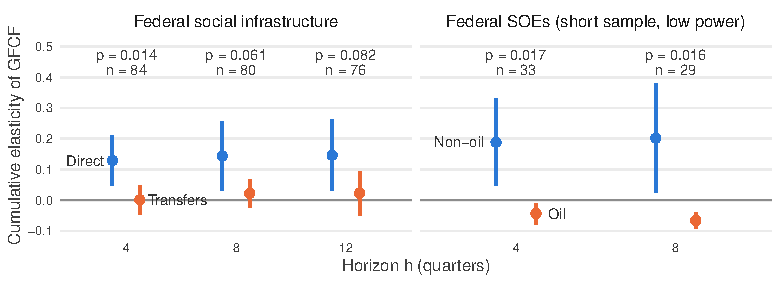
\includegraphics{figuras/A6_fig2_direta_transf_estatais.pdf}%
%{figuras/A6_fig2_direta_transf_estatais.pdf}
\caption{Joint local projections: cumulative elasticity of GFCF in volume with \CILevel\% intervals (Newey-West, small-sample correction); labels give the Wald $p$-value of equal coefficients and $n$. Left: federal social infrastructure, direct against transfers. Right: federal SOEs, non-oil against oil, from \SestOIStart.}
\label{fig:cmp}
\end{figure}

\textit{Local projections.} The dissertation aggregate has no significant effect on machinery and equipment (elasticity \LpInfElast, \LpInfElastLo{} to \LpInfElastHi, after \hC{} quarters, $n = \nLPC$) and a GFCF multiplier of \LpInfMult{} reais per real (\LpInfMultLo{} to \LpInfMultHi); direct federal investment in all functions has an elasticity of \LpGndElast{} (\LpGndElastLo{} to \LpGndElastHi{}) on machinery and equipment.

\textit{Comparisons.} We read the comparisons in elasticities from joint regressions (Table~\ref{tab:main}, panel B; Figure~\ref{fig:cmp}). Multipliers in reais say little about budget items that average \GshareSocDir\% (social, direct) to \GshareEconDir\% (economic, direct) of GFCF: the separate multiplier of social direct investment, \LpSocDirMultSep, falls to \LpSocDirMultJoint{} (\LpSocDirMultJointLo{} to \LpSocDirMultJointHi{}) in the joint regression. Economic and social infrastructure do not differ, with or without transfers ($p \geq \EcoSocpMin$ at every horizon and response). Within social infrastructure, direct investment raises GFCF more than transfers, \SocTrHAA{} against \SocTrHAB{} after \hA{} quarters ($p = \SocTrHAp$); the gap remains at \hB{} and \hC{} quarters only at the \SigLevelTen\% level ($p = \SocTrHBp$ and \SocTrHCp) and does not appear in machinery and equipment ($p$ from \SocTrMEpMin{} to \SocTrMEpMax). Among SOEs, non-oil investment has an elasticity of \SoeHAA{} against \SoeHAB{} for oil ($p = \SoeHAp$). With \SoeHAn{} observations and \SoeHAdf{} residual degrees of freedom the test has low power; the gap is not significant for machinery and equipment ($p = \SoeHAMEp$ and \SoeHBMEp). SOEs as a whole and direct federal investment do not differ significantly ($p$ from \SoeUnipMin{} to \SoeUnipMax). All intervals are pointwise: \NexclZero{} of \NcumTotal{} baseline cumulative elasticities exclude zero, where chance alone would give about \SigLevelTen\%.

\section{Next steps}

Part B moves to an annual panel of Brazilian states with Bartik-type shocks by type of investment. For the time series, the fragilities above set the agenda: the data do not settle the VAR-VEC choice, the oil split of SOEs has low power, and the gaps by modality and segment are absent from machinery and equipment.

\vspace{-3pt}
\begin{multicols}{2}
\raggedcolumns
\scriptsize
\renewcommand{\refname}{\normalsize References}
\begin{thebibliography}{99}

\bibitem[Andrews(1993)]{andrews1993}
Andrews, D. W. K. (1993). Tests for parameter instability and structural change with unknown change point. \textit{Econometrica}, 61(4), 821--856.

\bibitem[Bai and Perron(1998)]{bai1998}
Bai, J. and Perron, P. (1998). Estimating and testing linear models with multiple structural changes. \textit{Econometrica}, 66(1), 47--78.

\bibitem[Cavaliere et~al.(2012)]{cavaliere2012}
Cavaliere, G., Rahbek, A. and Taylor, A. M. R. (2012). Bootstrap determination of the co-integration rank in vector autoregressive models. \textit{Econometrica}, 80(4), 1721--1740.

\bibitem[Iasco-Pereira and Duregger(2023)]{iasco2023}
Iasco-Pereira, H. C. and Duregger, R. (2023). Public investment, infrastructure, and private investment in Brazil: is there a crowding-in effect? \textit{Economia}, ANPEC, 14, 1--19.

\bibitem[Jacinto and Ribeiro(1998)]{jacinto1998}
Jacinto, P. d. A. and Ribeiro, E. P. (1998). CO-INTEGRAÇÃO, EFEITOS CROWDING-IN E CROWDING-OUT ENTRE INVESTIMENTO PÚBLICO E PRIVADO NO BRASIL: 1973-1989. \textit{Revista Teoria e Evidência Econômica}, 6(11).

\bibitem[Johansen(1991)]{johansen1991}
Johansen, S. (1991). Estimation and hypothesis testing of cointegration vectors in Gaussian vector autoregressive models. \textit{Econometrica}, 59(6), 1551--1580.

\bibitem[Jord\`a(2005)]{jorda2005}
Jord\`a, \`O. (2005). Estimation and inference of impulse responses by local projections. \textit{American Economic Review}, 95(1), 161--182.

\bibitem[Oliveira(2020)]{oliveira2020}
Oliveira, R. N. d. (2020). \textit{Efeito crowding-out no Brasil}. Master's dissertation, Fundação Getúlio Vargas.

\bibitem[Ramey and Zubairy(2018)]{ramey2018}
Ramey, V. A. and Zubairy, S. (2018). Government spending multipliers in good times and in bad: evidence from US historical data. \textit{Journal of Political Economy}, 126(2), 850--901.

\bibitem[Reinsel and Ahn(1992)]{reinsel1992}
Reinsel, G. C. and Ahn, S. K. (1992). Vector autoregressive models with unit roots and reduced rank structure: estimation, likelihood ratio test, and forecasting. \textit{Journal of Time Series Analysis}, 13(4), 353--375.

\bibitem[Reis et~al.(2019)]{reis2019}
Reis, C. F. d. B., Araújo, E. C. d. and Gonzales, E. O. (2019). Public Investment Boosted Private Investment in Brazil between 1982 and 2013. \textit{Journal of Economic Issues}, 53(3), 813--840.

\bibitem[Zivot and Andrews(1992)]{zivot1992}
Zivot, E. and Andrews, D. W. K. (1992). Further evidence on the great crash, the oil-price shock, and the unit-root hypothesis. \textit{Journal of Business \& Economic Statistics}, 10(3), 251--270.

\end{thebibliography}
\end{multicols}

\end{document}
